\chapter{Results and discussion}

\textit{
In the previous chapter we described our main model and training procedure as well as some alternatives.
In this chapter we describe the numerical results of our implementation of the main model on two datasets, one synthetic dataset created from MNIST and the much more difficult Swedish population records. We also perform several experiments where we change the model configuration or training procedure and observe the effect on either or both datasets.
Hopefully, our observations can be instrumental in
% TODO: instrumental? Rephrase?
designing future encoder-decoder networks.
}

\section{Simulations on synthetic data} \label{sec:simulations}

Since the images of the Swedish records are so large, we decided to create a simpler and faster dataset so we could quickly iterate on the network architecture. Here we describe the synthetic dataset we created as well as some observations from altering the network configuration.

\subsection{Four-digit MNIST}


\begin{figure}
    \centering
    \begin{subfigure}[b]{0.45\textwidth}
        \centering
        
\includegraphics[scale=2.0]{resources/mnist4.jpg}
        \caption{Four digits without noise.
        %, size $112 \times 28$.
        }
        \label{fig:mnist4}
    \end{subfigure}%
    \begin{subfigure}[b]{0.45\textwidth}
        \centering
        
\includegraphics[scale=2.0]{resources/random_pad.jpg}
        \caption{Random position and dot noise.
        %Four digits with noise.
        %at a random position inside a box of $168 \times 56$ with dot noise.
        }
        \label{fig:mnist_random_pad}
    \end{subfigure}
    \caption{Two examples of generated synthetic data from MNIST.}
\end{figure}

For our early experiments we created a synthetic dataset with small images of four-digit sequences.
Each image was a concatenation of four independently randomly selected digit images from MNIST \cite{MNIST_orig}, where the first digit was always a one. See figure \ref{fig:mnist4} for an example. The resulting image was then a fixed size of $28 \times 112$ pixels.
%, compared to $900 \times 1500$ or more for the downsampled Swedish records.
% which is very much smaller than the images of the Swedish records.
Because the images were so small, it took a much shorter time to train and evaluate different models on the synthetic dataset than on the Swedish population records, whose images were very large.

Several models performed very well on this task, one of them achieving $94\%$ accuracy after 10,500 cpu-seconds of training. These models are discussed further in section \ref{sssec:exp_encoder}.

\subsection{Noisy MNIST}

In order to make the synthetic data a little bit more difficult to classify and more similar to the Swedish dataset, each four-digit image was placed at a random position in a larger image whose pixel values were zero, that is no ink.

When putting the four-digit image at a fixed position instead of a random position, one model learned to encode the distance from the left side of the image, which is quite interesting considering that neither the attention model nor the decoder had any explicit access to spatial information.
When adding $100$ additional zero-pixels to the right of the image, the accuracy dropped from $85\%$ to $80\%$. However, when adding $4$ zero-pixels to the left, the accuracy dropped to only $1\%$. We attribute this sudden accuracy loss to the difficulty of identifying which digit to keep and which to ignore. Since we are training on four-digit images but only expect the last three, the model must learn to find but ignore the first digit.
Since the year can appear at any position in the Swedish data, the simulations should also vary the position of the digits. Therefore, we must use random positions instead of fixed positions for the synthetic data.

Finally, we applied dot-noise to the image by:
(1) inverting the image so that the background is represented by one instead of zero,
(2) multiplying each pixel value with a random number drawn independently uniformly from $[0.6, 1.0]$ and
(3) inverting the image back again.
This corresponds to adding a random but small amount of ink to each pixel in the image.

An example image with dot noise and random position can be seen in figure \ref{fig:mnist_random_pad}. The models were evaluated on the image size $56 \times 168$ pixels, like in the figure.


\subsection{Network depth and width} \label{sssec:exp_encoder}

By running a time trace on the training operation, we saw that the majority of the training time was spent on applying and updating the encoder network. In order to reduce training time we performed the following experiments to design a more efficient encoder network while maintaining a good accuracy on the simulation tasks.
% TODO: insert graph?

% By counting the number of trainable parameters in the model we observed that the majority of parameters are contained by the MLPs in the attention and decoder model.

\subsubsection{Simulations on noise-free data}

Earlier in section \ref{sec:method_architecture} we presented a model architecture that we now refer to as DEP. We will come back to this model soon. In our initial experiments however we used another model for baseline, which we call DE. The DE encoder consisted of four blocks where the first three blocks contained two $3 \times 3$ convolutional layers and one $2 \times 2$ pooling layer. The last block contained a single $1 \times 5$ convolutional layer and one $1 \times 2$ pooling layer.
The main difference between DE and DEP is that DEP used one additional pooling layer between the two consecutive convolutional layers in the third block.
% The only difference between DEP and DE is that DEP had one additional pooling layer between two convolutional layers near the end of the encoder.
We will see that this small difference had a great impact on accuracy and running time.


\begin{figure}
    \centering
    \begin{subfigure}[c]{1.0\textwidth}
        \centering    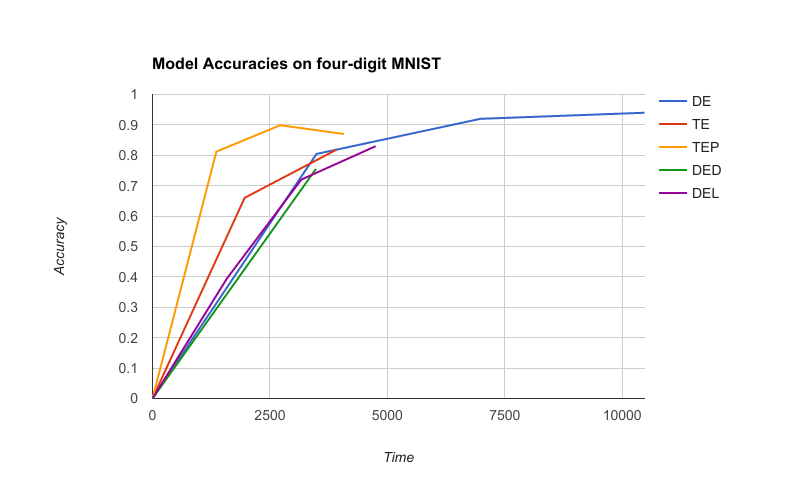
\includegraphics[scale=0.5]{resources/mnist_4_graph.png}
        \caption{Four-digit MNIST without noise.}
        \label{fig:mnist_early_models}
    \end{subfigure}
    \begin{subfigure}[c]{1.0\textwidth}
        \centering
        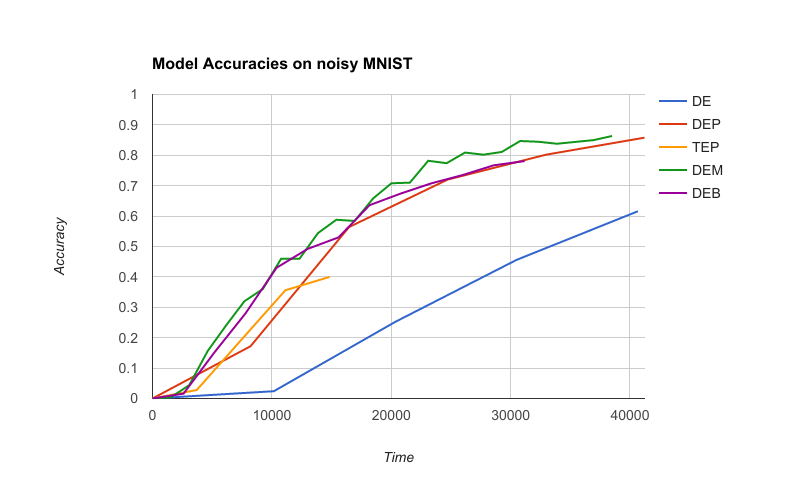
\includegraphics[scale=0.5]{resources/model_experiments.png}
        \caption{Noisy MNIST.}
        \label{fig:mnist_models}
    \end{subfigure}
    \caption{Plot of accuracy vs training time measured in CPU seconds for several models. Each data point comes after one epoch of training.}
\end{figure}


In figure \ref{fig:mnist_early_models} we can see the resulting accuracy over training time of the different variations of the DE model.
All configurations used cartesian loss (defined in section \ref{sssec:cartesian}) and soft attention (defined in section \ref{sssec:soft_attention}).

% For baseline we use a model called DE, which is rather similar to the model presented earlier in section

% The DE model was used as baseline with an encoder that had 7 layers and an output depth of 256. It is very similar to the DEP encoder illustrated in figure \ref{fig:encoder} except that it used one less pooling layer.

The model called DED was the same DE except that the decoder depth was halved from 1024 to 512. In figure \ref{fig:mnist_early_models} we can see that doing so had little impact on the accuracy and training time.

In another experiment, which we refer to as DEL, we halved the depth of every encoder layer. Halving the depth of every encoder layer halves the representational size in the encoder and consequently halves the training time. However, simplifying the encoder like this also seems to have limited its learning capability. In fact, it had about the same accuracy per training time as the DE model.

% When halving the depth of the DE decoder from 1024 to 512, (DED) had little impact on this task.
% Halving the number of filters in every layer (DEL) halved the training time per epoch but also halved the learning rate, so in the end its performance was about the same.

% The TE model was identical to DE except that it used fewer convolutional layers. More precisely, the DE encoder started with $\langle C,C,P,C,C,P \rangle$ while TE started with $\langle C, P, C, P \rangle$, where $C$ stands for $3 \times 3$ convolution and $P$ stands for $2 \times 2$ max-pooling.

% In both the DE model and the DEP model, the encoder had two consecutive convolutional layers at two places in the beginning of the encoder. These double layers in the DEP model can be seen in figure \ref{fig:encoder}.
In order to reduce the training time, we experimented with
simplifying the DE encoder by removing the second convolutional layer in each of the first two blocks. We call this thinner model TE.
% removing two convolutional layers so that there would be no consecutive convolutional layers. So in the model we call TE, every second layer in the encoder was a max-pool layer.
Similarly to the model DEL described above, where we simplified the encoder by halving the depth of each layer, both training time and accuracy was reduced. When plotting accuracy against training time in figure \ref{fig:mnist_early_models}, we see that just like DEL, the TE model was comparable to DE.

We also tested a variant to TE where an additional pooling layer was added between the two convolutional layers in the third block. So in this new model, which we call TEP, every second layer is a pooling layer.
Compared to TE, the TEP model learned much quicker. However, TEP started to overfit after hitting $90\%$ accuracy while the baseline model DE continued to improve until $94\%$.

% When adding an additional pooling layer (TEP) to the thinner model (TE), learning increased very rapidly for the first two epochs. However, it started to overfit after hitting $90\%$ accuracy, while the accuracy of the baseline model (DE) continued to rise to $94\%$.

In summary we can see that models with smaller representational size achieves about the same accuracy given the same amount of training time, although the heavier models seem to have higher potential in the long run. Another observation is that additional pooling can greatly increase the learning rate in the beginning of training.

% The learning rate on the simpler four-digit MNIST dataset for different some possible configurations of the encoder.

% By training on the simpler four-digit MNIST dataset without noise,
%we made several observations.
% We experimented on various configurations of encoder and decoder depth and width.
% we found that increasing the width of the decoder's hidden layer from 512 to 1024 had a very small impact on the training time while increasing accuracy. Decreasing the number of layers in the encoder from 7 to 5 decreased the accuracy somewhat but increased training time considerably. Halving the encoder width halved the training time but also decreased accuracy. Adding a pooling layer at the end of the encoder resulted in a higher accuracy after the first epoch and reduced training time. The effect of an extra pooling layer can be seen by comparing the models TE and TEP in figure \ref{fig:mnist_early_models}.

\subsubsection{Simulations on noisy data}

The best configurations so far were evaluated on the more difficult synthetic dataset with random positions and noise. Figure \ref{fig:mnist_models} contains a comparison between some variations of encoder configurations on the noisy MNIST dataset.
By comparing this graph to figure \ref{fig:mnist_early_models}, we can see that using larger input images, placing the digits at a random position and adding noise makes the problem much more difficult. Training a single epoch takes almost three times as long and the increase in accuracy per epoch is reduced considerably.
%Note that for the same model, we needed to train more than 4 times longer to get the same accuracy as on the simpler synthetic dataset.

The three best configurations (DEP, DEB, DEM) achieved very similar results considering the test accuracy vs training time. These three configurations had the same number of encoder layers but different depth of each layer.

The heaviest encoder DEP is illustrated in figure \ref{fig:encoder}.
Because it had the most number of filters, the training time for each epoch was much longer than for the other two alternatives.
% For this encoder the representational size of the input decreases exponentially for each pooling layer: 32, 16, 8, 4, 2.
Since each pooling layer divides the representational size by four and the number of filters in this model doubles after almost every pooling layer, the representational size decreases is halved after most pooling layers.

While the representational size decreases for DEP, as recommended by \textcite{InceptionV3}, the DEM encoder was designed to keep the representational size as constant as possible from the start.
This was done by reducing the layer depth to a minimal amount, with only 4 filters at the input layer instead of 32.
As we can see in figure \ref{fig:mnist_models}, the training time for each epoch was much faster although the actual learning over time was almost the same as for the DEP model.

The third competing encoder DEB was a middle ground between DEP and DEM, designed to have a very slowly decreasing representational size.

\subsubsection{Wider encoders are more robust to varying input size}


\begin{figure}
    \centering
    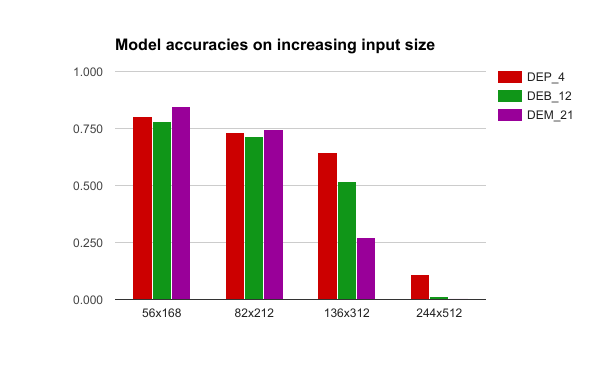
\includegraphics[scale=0.5]{resources/mnist_resilience.png}
    \caption{Noise resilience... TODO}
    \label{fig:mnist_resilience}
\end{figure}

When increasing the size of the generated synthetic images without retraining the models, the accuracy of the DEP model was relatively stable even for the double width and height but dropped for larger input. The two lighter models, DEB and DEM, were less robust to this change in input; see figure \ref{fig:mnist_resilience}.

The attention model is responsible for choosing the correct location in the input image. The receptive field of output units in the three configurations were the same and the architecture of the attention model was identical. The background noise was also identical. So although the attention model worked well for a smaller image, it is not sure it may work as well for a larger image where the background is the same.
% One possible reason for this is that the soft attention for all locations must sum to one. Since there are more locations to choose from, the weight on the correct location decreases.
Remember that the attention model does not know how many locations there are but outputs a salience score for each location independently. Since we use the softmax of these salience scores, the resulting attention weights must sum to one. So the more locations there are, the more the attention risk to spread out over noisy locations. To counter this, the attention model would have to be even more aggressive to separate background noise from useful signals. For hard attention however, only the most promising location is kept and the rest are ignored. So a model trained with hard attention should be more resilient to increased image size. We discuss more about attention later in section \ref{sssec:result_attention}.

We see that the more filters a model has, the more stable it is to change. Hence we believe that although on a single task the three configurations performed comparatively, the heavier model generalizes better in the long run.

% We attribute this resilience to noise to detecting more features in the input, some of which are better preserved after adding the noise.


% We argue that the heavier model, DEP, with its additional filters can detect more features in the input

% The lightest encoder (DEM) was designed to have the same representational size as DEP at the end of the encoder but decreasing the number of filters in the beginning in order
% keeping the representational size as constant as possible from the start by using fewer filters, in contrast to the advice from \textcite{InceptionV3}.


\section{Experiments on Swedish population records} \label{sec:experiments}

In this section we present and discuss our model with variations on the Swedish population records.
% metrics of different models and training
% comparisons we made between different models on the Swedish population records.

\subsection{Setup}
 Here we describe the platform on which we evaluated the models.

\subsubsection{Downsampling}
The images of the Swedish population records had a high resolution so they were downsampled with a ratio of 8. For example instead of having a size of $4688 \times 6360$ an image would have the size to $586 \times 795$. Because the images have different sizes, in each batch the images were padded with zeroes to get the same size as the largest image in the batch.

\subsubsection{Implementation}
The models were implemented in Tensorflow \cite{Tensorflow}, which is a popular open-sourced machine learning framework. The implementation\footnote{\url{https://github.com/HalfLeif/CNN_doc_extraction}} is freely available on Github.

\subsubsection{Hardware}
We trained the models on 3 threads on a single Intel(R) Core(TM) i7-4770K @ 3.50GHz. Training a single epoch of Swedish population records took about 28 hours. It would be faster to train using more threads or GPU acceleration but we were constrained by limited access to hardware.


\subsubsection{Pre-training}

All experiments in this section start with a pre-trained model already. Most of them use a model we refer to as the \textbf{base model}. The base model used the DEP encoder and was trained using soft attention and cartesian loss for 5 epochs on the noisy MNIST and then for 16 epochs on the Swedish population data. Thus it had an accumulated training time of more than 4,200,000 cpu-seconds or almost 3 weeks on our hardware.
% noisy MNIST DEP-5: 41,217 cpusec ?
% 16 epochs of SweDEP: 264775*16 cpusec = 4,236,400
% SUM:
The base model had an accuracy of $8.39\%$ on the main test set and an accuracy of $2.11\%$ on the second test set.

Optimally, the model variations should be retrained from scratch but doing so would simply take too long time.
Instead, we present the observed accuracies as a lower bound to the potential of each observation and as an indication of whether the variation was helpful or not.
% Since the models were heavily pre-trained with a different configuration, we present our observations as a lower bound to the potential accuracy of each variation.

% that pre-trained on the noisy MNIST for 5 epochs which was then trained on the Swedish population data

% The experiments in this section were performed after training the model for many epochs on the Swedish data already. Optimally we would want to retrain the model from scratch for each alteration but doing so would take too much time. Thus we can only provide a lower bound for the accuracy of the altered models.


\subsection{Independent digits vs cartesian loss} \label{sssec:ind_digits}

We now compare using the independent digit loss presented in section \ref{ssec:method_loss} against the cartesian loss introduced in section \ref{sssec:cartesian}.
% TODO: check in notes for results on MNIST data.
Training the DEP configuration from scratch on the noisy MNIST data using either loss function gave very similar results although the training time was slightly longer for cartesian loss.

For the Swedish population records, the base model used cartesian loss already. When training one additional epoch using the independent digit loss, the test accuracy dropped from $8.39\%$ to $7.2\%$. However, when training the model for another six epochs we reached the test accuracy of $8.98\%$. This model we refer to as base2 because some of the following models were trained from this model.

\subsection{Multi-year vs single-year loss} \label{ssec:result_multiyear}

Both the cartesian loss and independent digit loss discussed above only used a single year from the label. We suggested another loss function in section \ref{sssec:alt_multiyear} that takes into account the full year interval in the label by averaging the loss function over all years in the label interval. Now we compare using the multi-year vs the single-year version of independent digit loss.

As mentioned above, when changing the loss function for the base model to single-year independent digit loss for one epoch, the accuracy dropped from $8.39\%$ to $7.2\%$. However, when instead changing it to the multi-year version, the accuracy dropped even further to $7.07\%$. When training with multi-year loss from base2 for four epochs, the test accuracy dropped from $8.98\%$ to $7.58\%$

Although the test accuracy for the multi-year model decreased, the accuracy on the second test set increased from $2.35\%$ to $2.75\%$. This is the best result we have achieved on the second test set, which tests the model on completely new books from other regions.

% TODO: insert table of accuracies on both test sets for different variations. Can use two different tables for single epoch and multi epoch additional training.

\subsection{Simplifying the training data}

When a page contains multiple valid years, our single-year loss function only rewards finding the highest year and penalizes all other years, including valid ones.
In our previous experiment, we attacked this problem of miss labeling in our training data by making a loss function that takes into account all the years in the label. In this experiment, we instead try to estimate the impact of miss labeling by only training on images that have a single year in it. Here we again the use single-year independent digit loss function.

After training for one additional epoch beyond the base2 model, the test accuracy dropped from $8.98\%$ to $8.83\%$.
After another five epochs, we reached the highest seen test accuracy of $9.54\%$. On the other hand, the accuracy on the second test set was an all-time low at $1.42\%$.

\subsection{Soft vs hard attention} \label{sssec:result_attention}

So far, all reported models have used soft attention. Hard attention uses the same network, the only difference is that instead of doing a weighted sum over the encoded locations, we choose one of them. In previous work, the hard attention has seen the attention weights as a distribution over the location and samples that distribution. In our work however, we simply choose the location with highest attention weight.


\begin{figure}
    \centering
    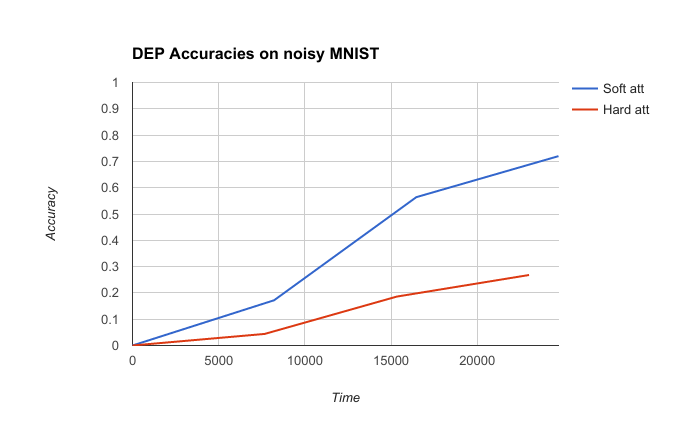
\includegraphics[scale=0.6]{resources/soft_vs_hard.png}
    \caption{The DEP model learns much faster with soft attention on the noisy MNIST dataset. Plot of accuracy vs training time measured in CPU seconds.}
    \label{fig:attention_mnist_graph}
\end{figure}


When training the DEP model with hard attention from scratch on the noisy MNIST data for one epoch, we only got a test accuracy of $4.4\%$ instead of $17.2\%$.
In figure \ref{fig:attention_mnist_graph} we can see how much quicker the DEP model learns to recognize digit sequences using soft attention.


\begin{figure}
    \centering
    \begin{subfigure}[c]{0.45\textwidth}
        \centering    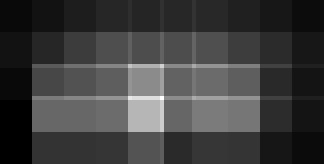
\includegraphics[scale=2.0]{resources/MNIST_soft_att/1177_att.jpg}
        \caption{Soft attention in white on the image to the right. It correctly focused more to the bottom and left.}
        % \label{fig:mnist_early_models}
    \end{subfigure} \quad %
    \begin{subfigure}[c]{0.45\textwidth}
        \centering
        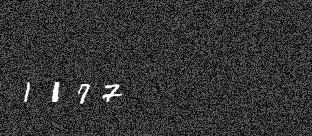
\includegraphics[scale=2.0]{resources/MNIST_soft_att/1177_correct.jpg}
        \caption{The image was correctly classified as 1177.}
        % \label{fig:mnist_models}
    \end{subfigure}
    
    \vspace{1em}
    
    \begin{subfigure}[c]{0.45\textwidth}
        \centering    
\includegraphics[scale=2.0]{resources/MNIST_hard_att/1281_att.jpg}
        \caption{Hard attention in white of the image to the right. The attention only captured part of the number.}
        % \label{fig:mnist_early_models}
    \end{subfigure} \quad %
    \begin{subfigure}[c]{0.45\textwidth}
        \centering
        
\includegraphics[scale=2.0]{resources/MNIST_hard_att/1281_fail_1031.jpg}
        \caption{Input image with label 1281, it was incorrectly classified as 1031.}
        % \label{fig:mnist_models}
    \end{subfigure}
    \caption{Examples of soft and hard attention applied to noisy MNIST images with sizes $312 \times 136$.}
    \label{fig:attention_mnist}
\end{figure}


In figure \ref{fig:attention_mnist} we can see how the soft attention successfully captured the year by putting together information from several locations. In the same figure, the hard attention fails because it can only see some of the digits.

When training the base model for one epoch with hard attention on the Swedish population records, the accuracy dropped from $8.39\%$ to $2.19\%$.


\begin{figure}
    \centering
    \begin{subfigure}[c]{1.0\textwidth}
        \centering    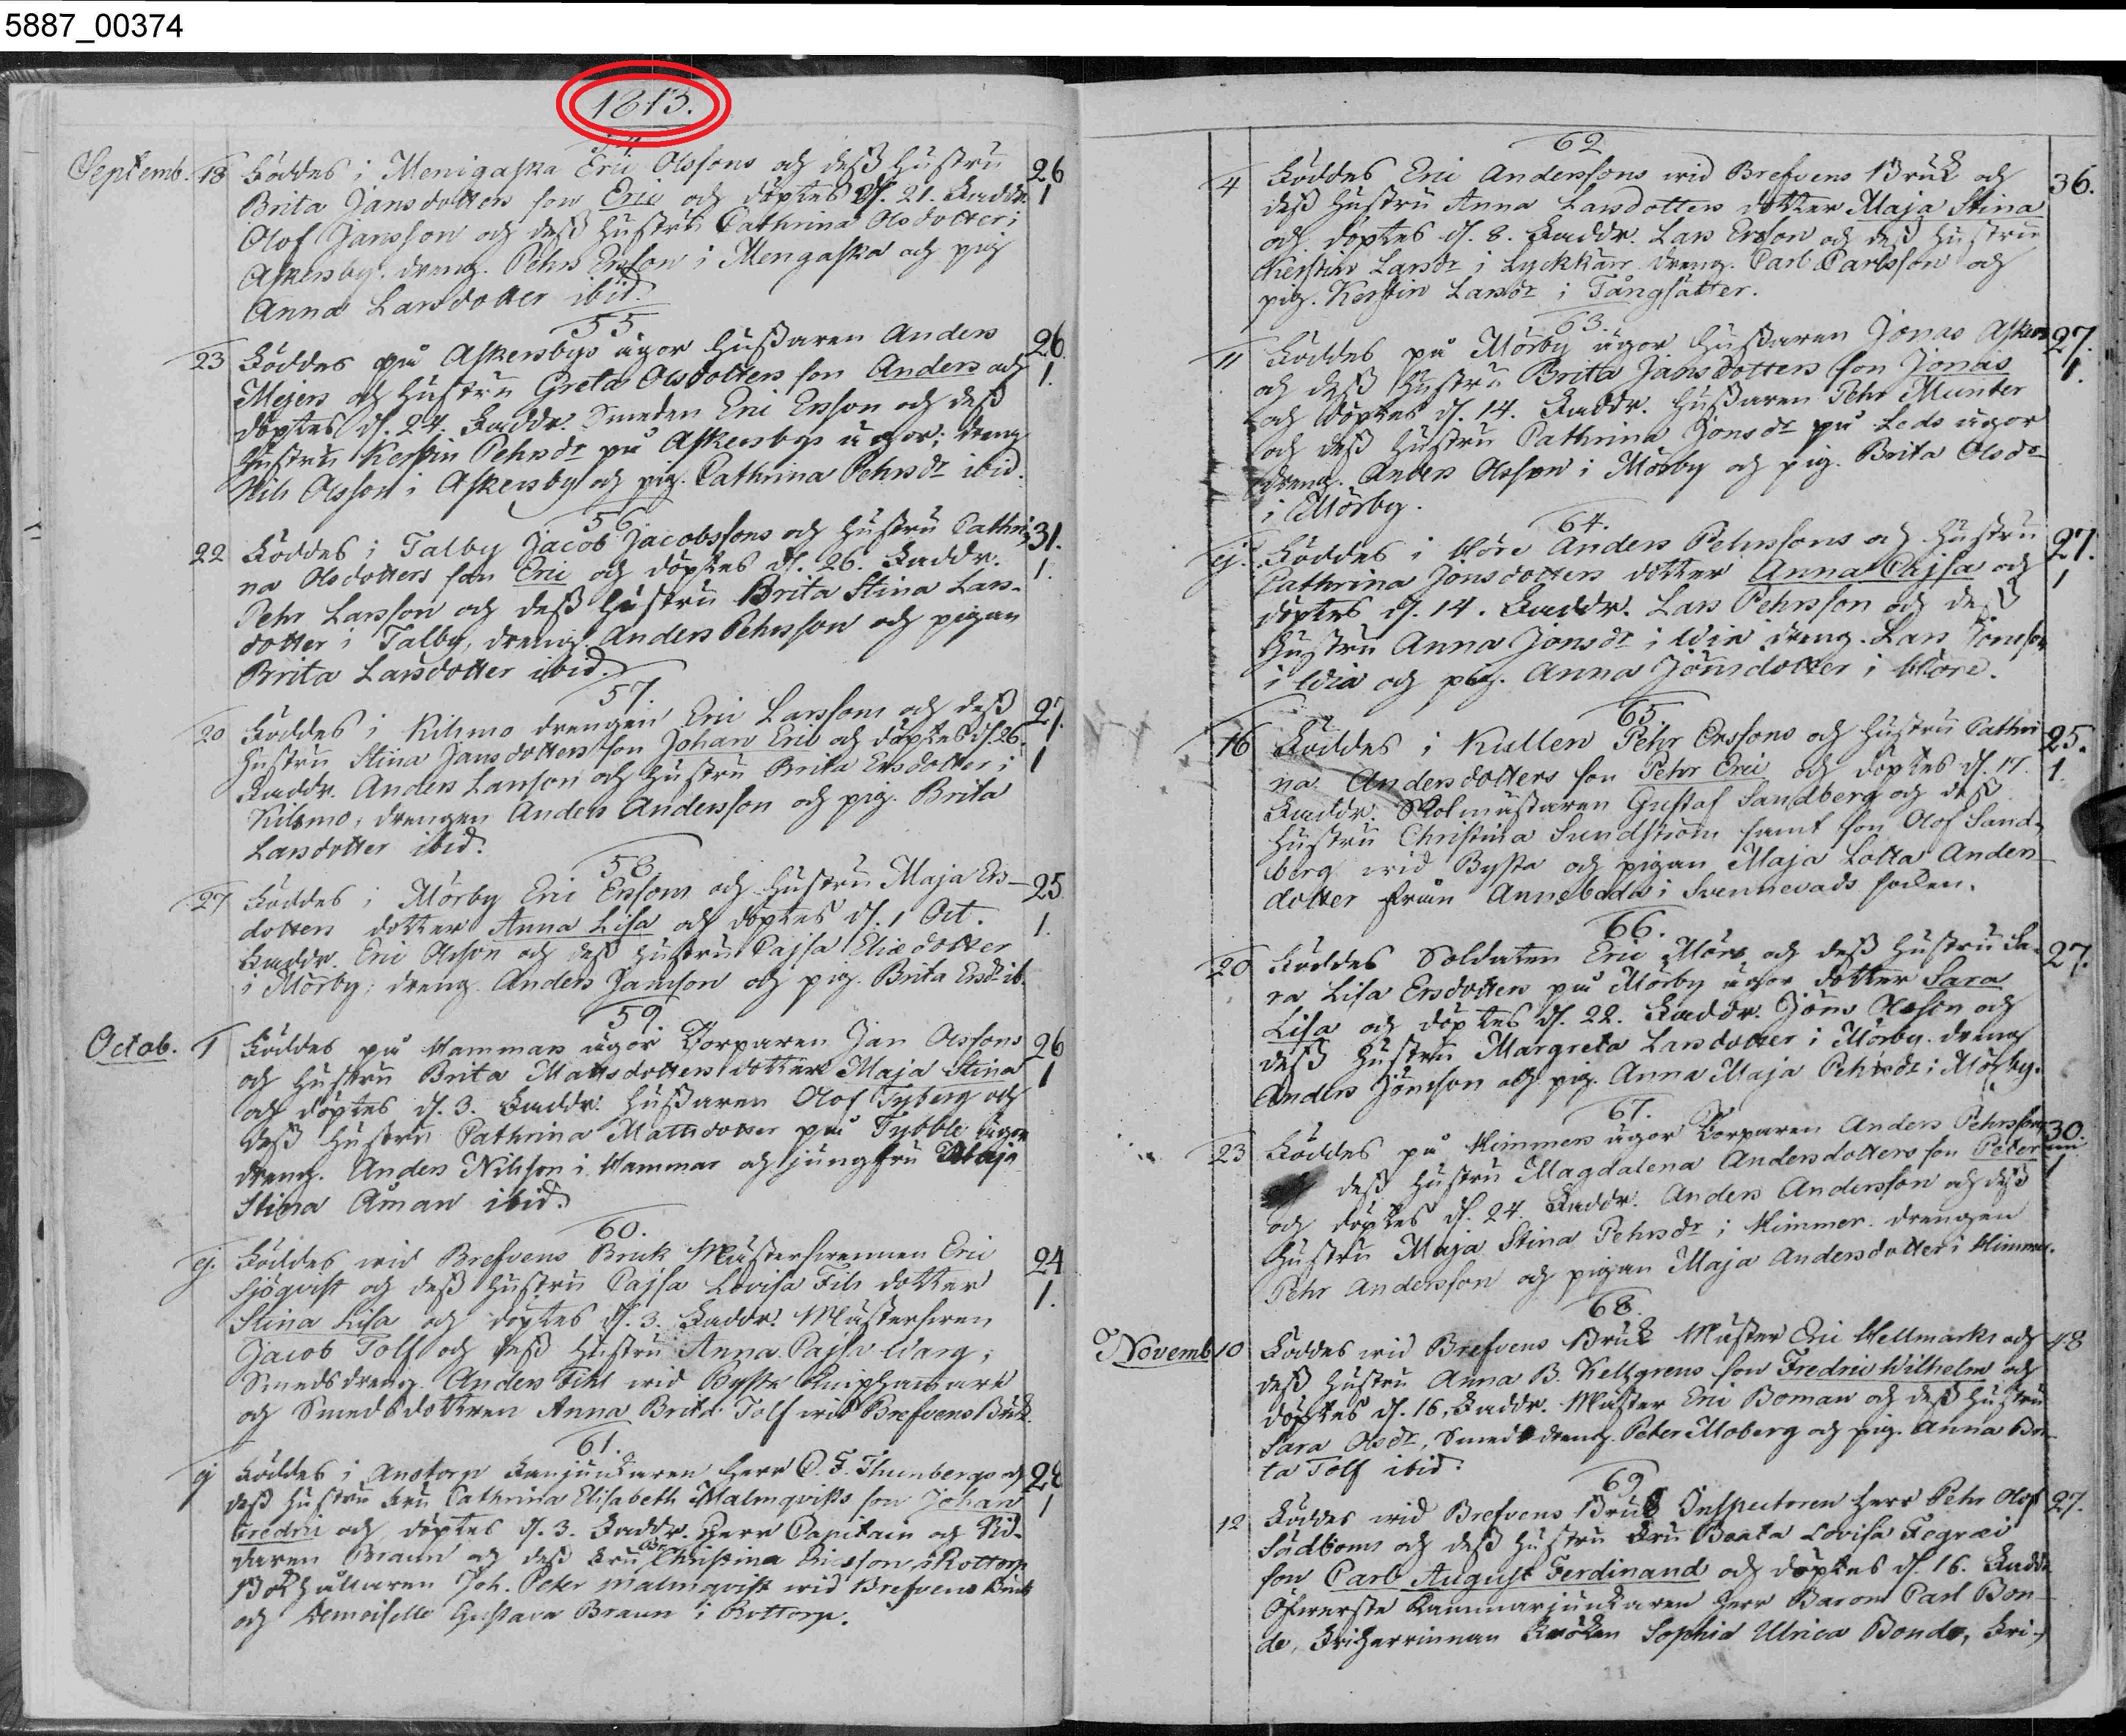
\includegraphics[scale=0.56]{resources/SWE_attention/S3HT-64P3-T61.jpg}
        \caption{The correct year is 1813; it is emphasized in the picture with ellipses.}
    \end{subfigure}
    
    \vspace{1em}
    
    \begin{subfigure}[t]{0.45\textwidth}
        \centering
        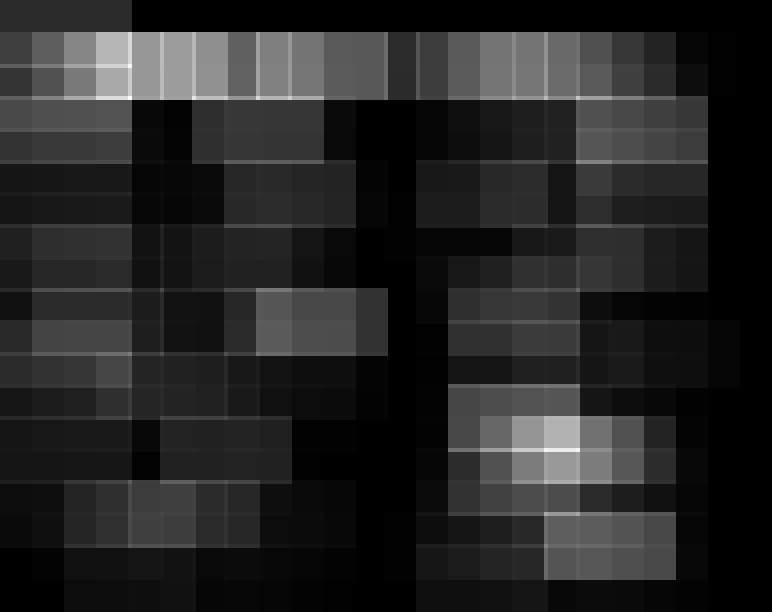
\includegraphics[scale=1.0]{resources/SWE_attention/SoftAtt/att_S3HT-64P3-T61.jpg}
        \caption{The base model correctly classifies the image as 1813. The attention correctly focuses on the year as well as on some handwriting.}
    \end{subfigure} \quad %
    \begin{subfigure}[t]{0.45\textwidth}
        \centering    
\includegraphics[scale=1.0]{resources/SWE_attention/HardAtt/att_S3HT-64P3-T61.jpg}
        \caption{The hard attention model predicts the page as 1899 because it is looking at the wrong location.}
    \end{subfigure}
    
    \caption{An image from the main test collection. The page comes from the book Asker C:4 in the Örebro collection.}
    \label{fig:attention_dep_T61}
\end{figure}


\begin{figure}
    \centering
    \begin{subfigure}[c]{1.0\textwidth}
        \centering    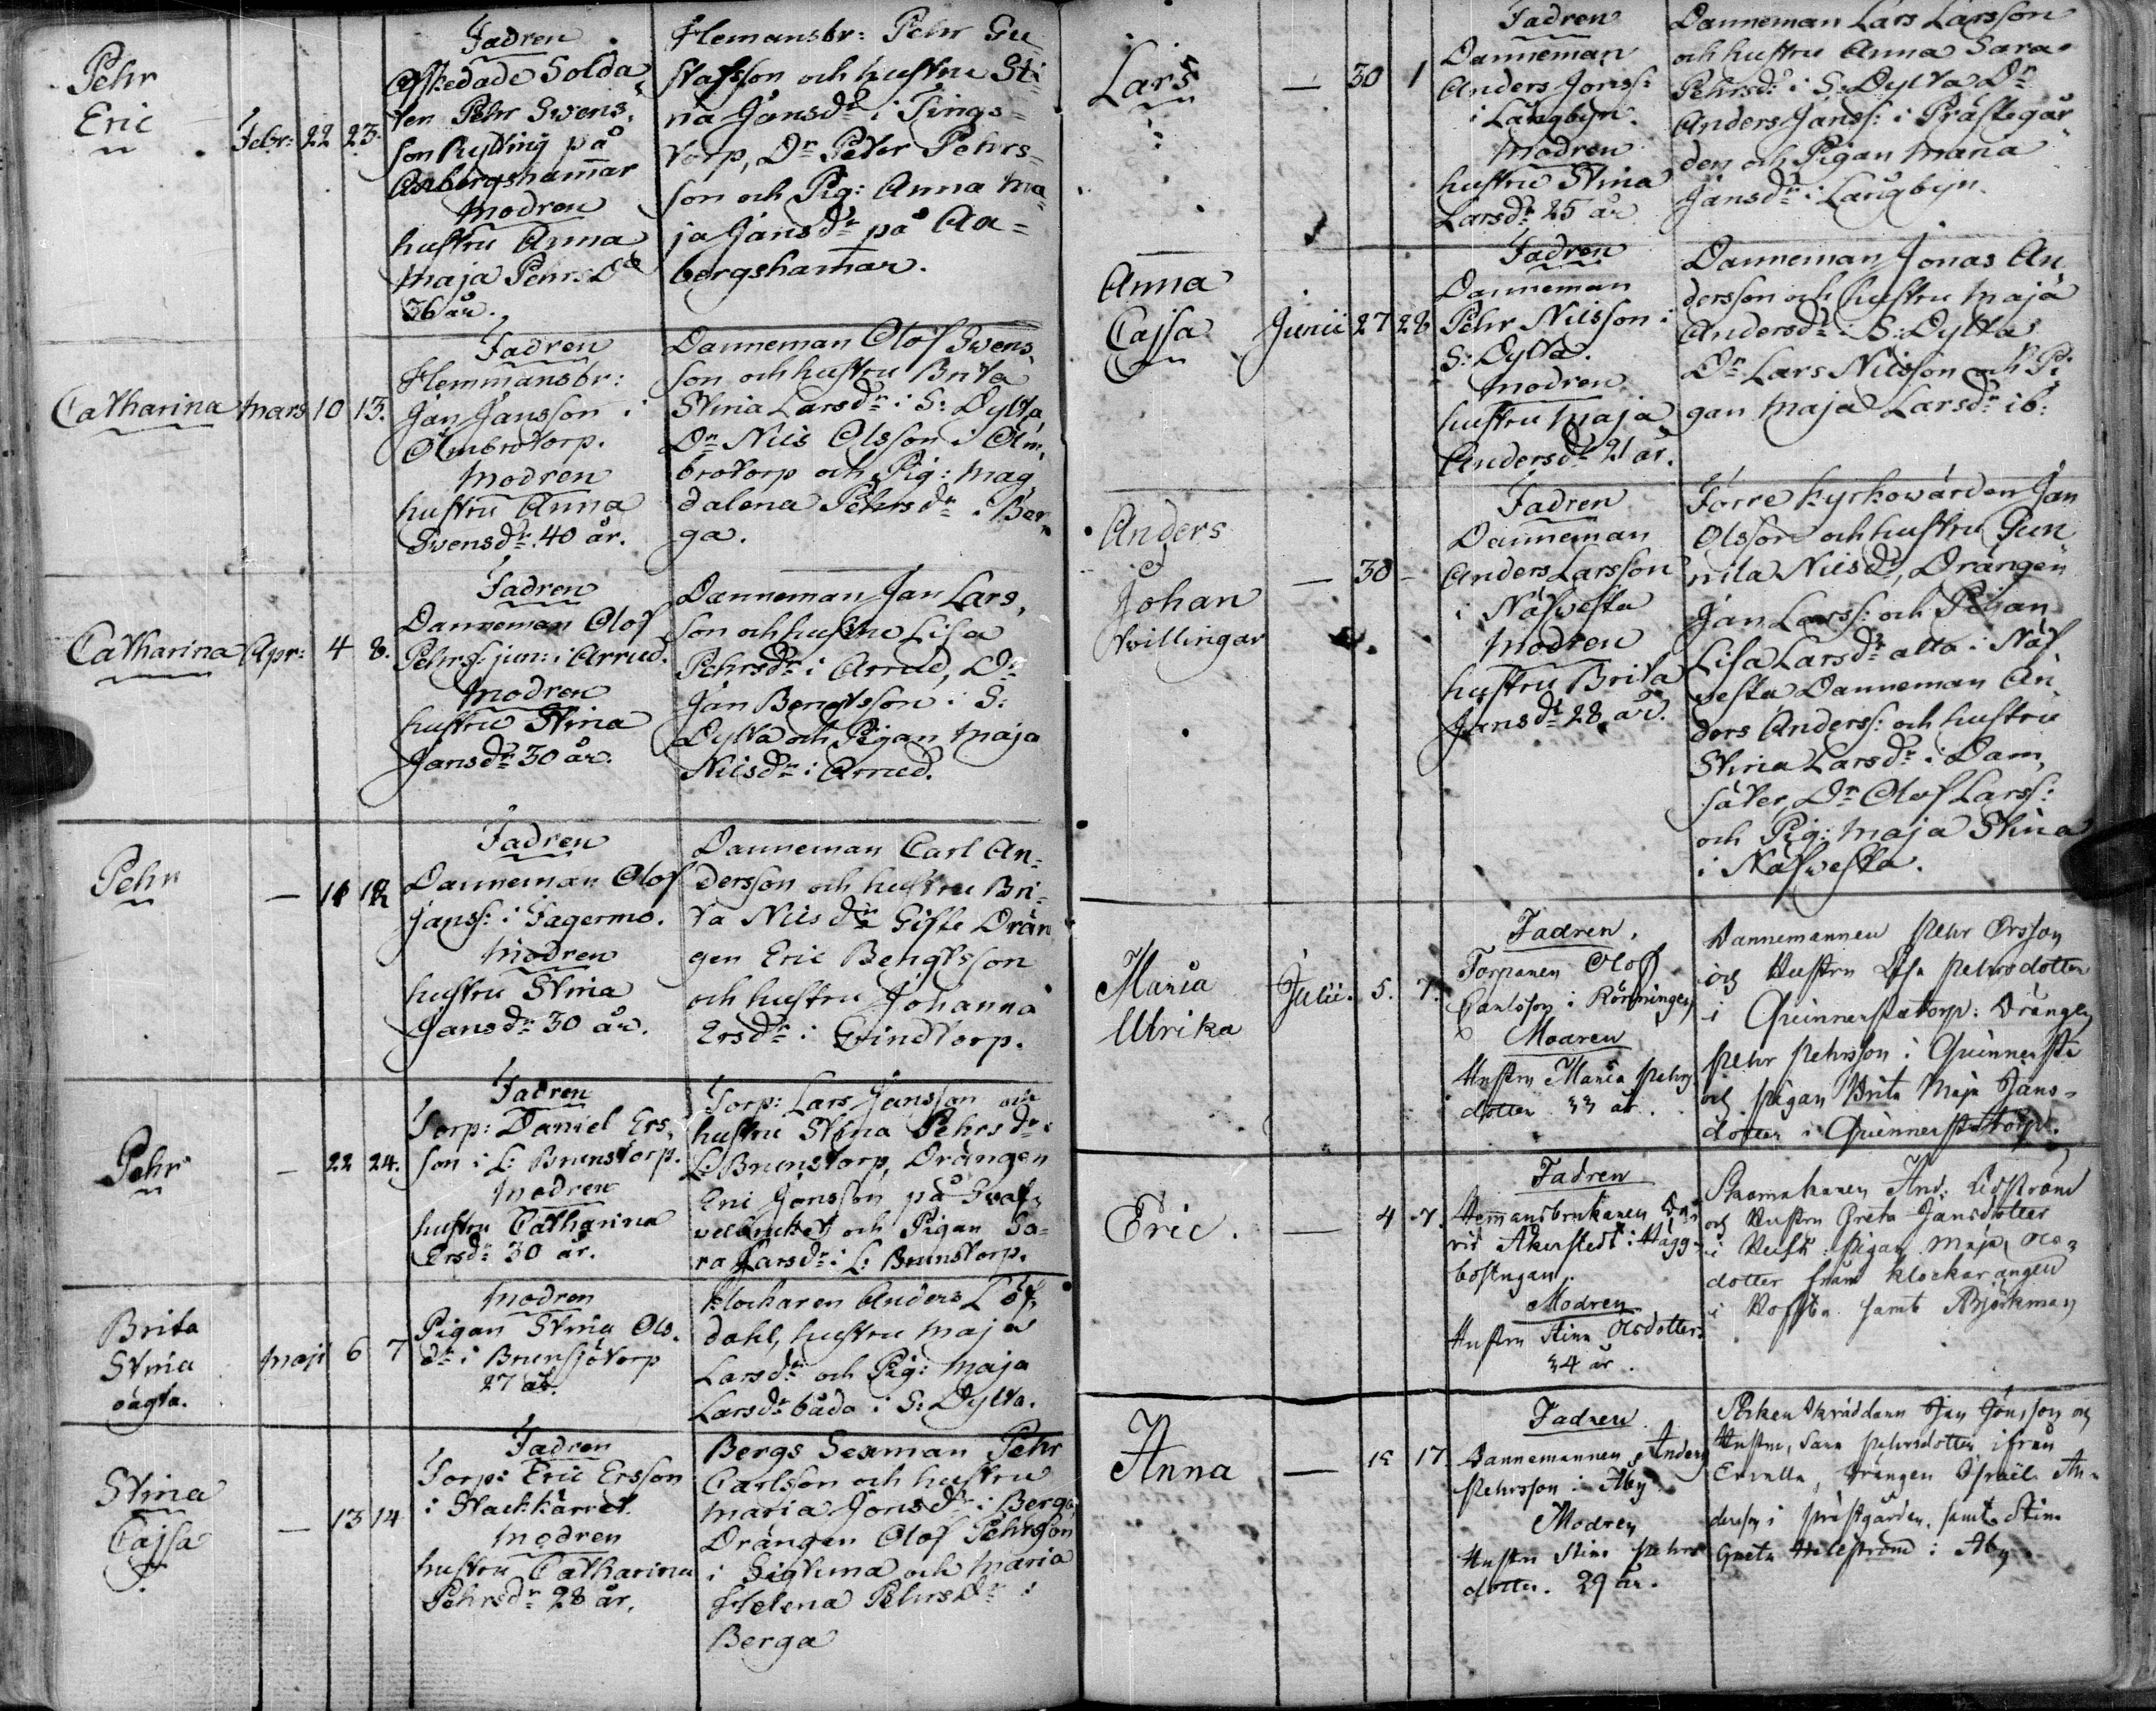
\includegraphics[scale=0.29]{resources/SWE_attention/S3HY-DRC3-H5L.jpg}
        \caption{The correct year is 1814, although the year is actually not written in the page but inferred from previous pages.}
    \end{subfigure}

    \vspace{1em}

    \begin{subfigure}[t]{0.45\textwidth}
        \centering
        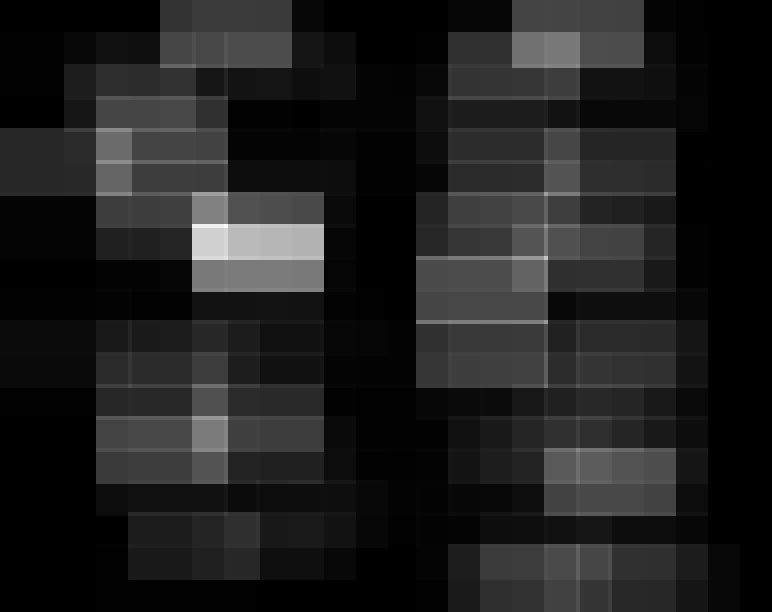
\includegraphics[scale=1.0]{resources/SWE_attention/SoftAtt/att_S3HY-DRC3-H5L.jpg}
        \caption{The base model classifies the image as 1811 by looking at the handwriting.}
    \end{subfigure} \quad %
    \begin{subfigure}[t]{0.45\textwidth}
        \centering    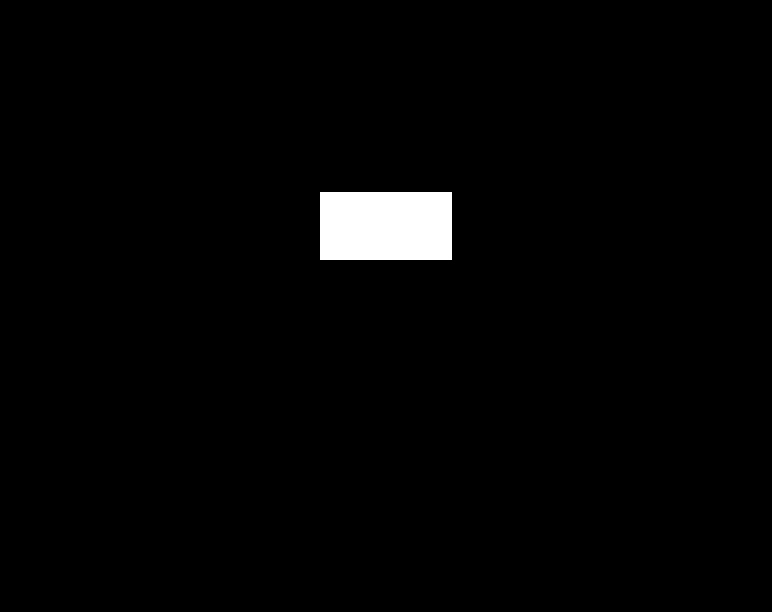
\includegraphics[scale=1.0]{resources/SWE_attention/HardAtt/att_S3HY-DRC3-H5L.jpg}
        \caption{The hard attention model predicts the page as 1760.}
    \end{subfigure}

    \caption{Soft vs Hard attention on an image from the main test collection. The page comes from the book Axberg C:5 in the Örebro collection.}
    \label{fig:attention_dep_H5L}
\end{figure}


\section{Post-processing} \label{sec:result_post_process}

The best result on the second dataset had an accuracy of $2.75\%$, using multi-year loss. When running the post-processing on the predictions of this model, the accuracy was increased to $3.58\%$. So even though the original predictions were quite noisy, the post-processing could still use them to boost the accuracy further.

We also tested the post-processing on the indexed part of the Örebro collection. Note that this collection was partitioned for both training and testing, so $90\%$ of the predictions are on training data. The accuracy of base2 was $14.9\%$ on this collection. Post-processing increased the accuracy to $15.9\%$. The mean distance between the prediction and the label was also reduced from 6 years to 4 years after post-processing.

% Works Örebro, Asker-C-2 189:
% 	 S3HT-64P3-KY5 1768 1768 [1768]
% 	 S3HT-64P3-PS4 1768 1768 [1768, 1769]
% 	 S3HT-64P3-KTG 1768 1768 [1769]
% 	 S3HT-64P3-T3Q 1771 1769 [1769]
% 	 S3HT-64P3-R81 1771 1770 [1769]
% 	 S3HT-64P3-V2C 1777 1771 [1769]

% Fail Asker-C-3 147:
% 	 S3HT-64P3-2W5 1798 1798 [1797]
% 	 S3HT-64P3-T75 1795 1798 [1797]
% 	 S3HT-64P3-NXY 1798 1798 [1797, 1798]
% 	 S3HT-64P3-233 1798 1798 [1798]
% 	 S3HT-64P3-KRW 1805 1808 [1798]
% 	 S3HT-64P3-RZP 1798 1808 [1798]

\begin{table}
\begin{subtable}{\linewidth}
\centering
\begin{tabular}{|c|c|l|}
    \hline
    Before & After & Correct \\
    \hline
    1768 & 1768 & 1768 \\
    1768 & 1768 & 1768, 1769 \\
    1768 & 1768 & 1769 \\
    1771 & \textbf{1769} & 1769 \\
    1771 & 1770 & 1769 \\
    1777 & 1771 & 1769 \\
    \hline
\end{tabular}
\caption{The post-processing can correct one of the pages to 1769. Although 1771 is not correct for the last page in the example, it is still closer to the true value than the prediction 1777.
}
\end{subtable}

\vspace{1em}

\begin{subtable}{\linewidth}
\centering
\begin{tabular}{|c|c|l|}
    \hline
    Before & After & Correct \\
    \hline
%   \textbf{h [m} & \textbf{dim [m} \\ \hline
    1798 & 1798 & 1797 \\
    1795 & 1798 & 1797 \\
    1798 & 1798 & 1797, 1798 \\
    1798 & 1798 & 1798 \\
    1805 & \textbf{1808} & 1798 \\
    1798 & 1808 & 1798 \\
    \hline
\end{tabular}
\caption{
The network makes a confident but incorrect prediction that the century digit should be 8 and the decade digit 0. The incorrect prediction makes the post-processing prefer 1808 over the true value of 1798.
}
\end{subtable}
\caption{Two examples of post-processing. In the column to the left is the prediction made by the model, the middle column contains the updated prediction after post-processing and the rightmost column contains the true label. The first example comes from the book Asker C:2 and the second from Asker C:3, both from the Örebro collection.}
\label{tab:post_process_example}
\end{table}


In table \ref{tab:post_process_example} we can see some examples of the post-processing applied to books in the Örebro collection. The post-processed sequence is typically very smooth compared to the raw predictions. Sometimes a single confident but incorrect prediction can start a long sequence of errors. One of the reasons for this is that the jump distribution strongly prefers increasing the year over decreasing the year.

\subsection{Jump distribution}


\begin{figure}
    \centering
    \begin{subfigure}[c]{1.0\textwidth}
        \centering        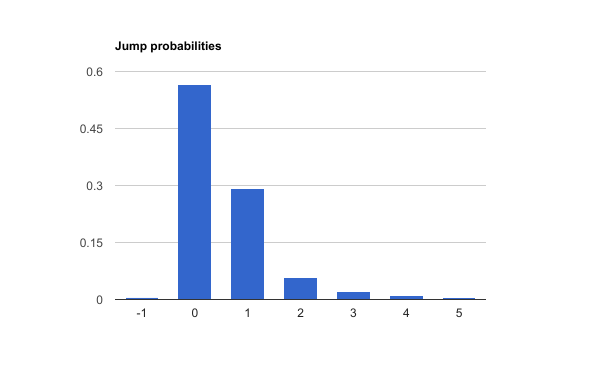
\includegraphics[scale=0.7]{resources/jump_distribution.png}
        \caption{As expected, the following page is most likely the same year or the consecutive year. With laplace smoothing of $0.5$, the probability for a zero-transition is $56.5\%$ and the probability for a plus-one-transition is $29.1\%$. The interval $[-1,5]$ contains $95.5\%$ of the smoothed distribution.}
        \label{fig:jump_prob}
    \end{subfigure}
    \begin{subfigure}[c]{1.0\textwidth}
        \centering
        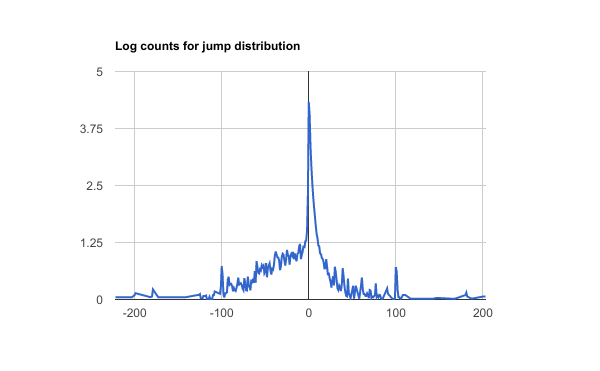
\includegraphics[scale=0.7]{resources/jump_log_counts.png}
        \caption{The plot shows $\log(1+\text{count}(x))$ for each label transition $x$.}
        \label{fig:jump_log_counts}
    \end{subfigure}
    \caption{The jump probability calculated from the training set and main test set.}
\end{figure}


The major chunk of the jump probability distribution is illustrated in figure \ref{fig:jump_prob}. We see that most page transitions should either keep the same year or increase by one.
As described earlier in section \ref{sssec:alt_postproc}, when counting transitions between two pages where both pages have multiple years, we give fractions of count to all combinations of years. This results in the small probabilities for minus one and plus two et cetera, which can be seen in the probability distribution.
% Because of multi-year labels, we also have small probabilities for minus one and plus two, since we count all combinations of .

It also happens in some books that there is a major leap between two pages as a new section of the book begins. This can be seen in the log counts for the four main collections of the Swedish population records, which is plotted in figure \ref{fig:jump_log_counts}.

\subsection{Conditional jump distribution}
One problem with the above jump distribution is that, for our dataset, a vast majority of the page transitions are zero jumps; that is from the same label to itself.
Because the distribution heavily favors the zero jump, the predictions after post-processing often output the same year for all pages in a book, instead of increasing years as we would expect.

One idea to fix this is to condition the current transition on the previous transition. The idea is that if the previous transition was a zero jump, we should be more likely to change year now. However, when aggregating the statistics for the Swedish dataset, it turns out our intuition was wrong: if the previous transition was a zero jump, it is even greater probability that the current transition is a zero jump. So a conditional distribution reinforces the problem instead of alleviating it.


\section{Model comparison}

%  & Swe_DEP_7-199 & 0.0417 & 10 & 18 & 0.262 &  &  &  &

\begin{table}
  \centering
  \begin{tabular}{|c|c||c|c|c|c||c|c|c|c|}
    \hline
    & & \multicolumn{4}{c||}{Main} & \multicolumn{4}{c|}{Secondary} \\
    % \hline
    Name & Epochs & Acc & Med & Mean & Near & Acc & Med & Mean & Near \\
    \hline
    Base & 16 & 0.0839 & 6 & 10 & 0.408 & 0.0211 & 23 & 30 & 0.113 \\
    \hline
    Ind & 16+1 & 0.0720 & 6 & 11 & 0.423 & 0.0221 & 21 & 29 & 0.129 \\
    & 16+6 & 0.0850 & 6 & 10 & 0.436 & 0.0211 & 24 & 31 & 0.111 \\
    (Base2) & 16+7 & 0.0898 & 6 & 10 & 0.429 & 0.0235 & 26 & 33 & 0.115 \\
    \hline
    Multi & 16+1 & 0.0707 & 6 & 10 & 0.400 & 0.0157 & 26 & 33 & 0.104 \\
    & 23+4 & 0.0758 & 6 & 11 & 0.410 & 0.0275 & 21 & 29 & 0.130 \\
    +post & 23+4 & & & & & \textbf{0.0358} & 18 & 28 & 0.156 \\
    \hline
    Simple & 23+1 & 0.0883 & 6 & 10 & 0.426 & 0.0216 & 25 & 31 & 0.120 \\
    & 23+6 & \textbf{0.0954} & 6 & 10 & 0.431 & 0.0142 & 26 & 32 & 0.100 \\
    \hline
    Hard & 16+1 & 0.0219 & 20 & 35 & 0.150 & 0.0152 & 32 & 41 & 0.097 \\
    \hline
  \end{tabular}
  \caption{For each model, we list for how many epochs it has been trained including pre-training, four metrics on the main test set and four metrics on the second test set for generalization.
  The first metric is accuracy, the second is median distance between prediction and correct label, the third is the mean distance and the last metric is the percentage of predictions that were less than 5 years wrong from the correct label.
  The models are the Base model, independent digit loss, multi-year loss, multi-year loss with post-processing, simplified training data and hard attention.
  Note that the models that are pre-trained with 16 epochs use the Base model, while the models that are pre-trained with 23 epochs use the Base2 model.
  }
  \label{tab:model_overview}
\end{table}


TODO: compare metrics and suggest best model. Also show confidence thresholds?

\section{What has the model learned?}

\begin{figure}
    \centering
    \begin{subfigure}[c]{1.0\textwidth}
        \centering
        % img_S3HT-64P3-2GW
        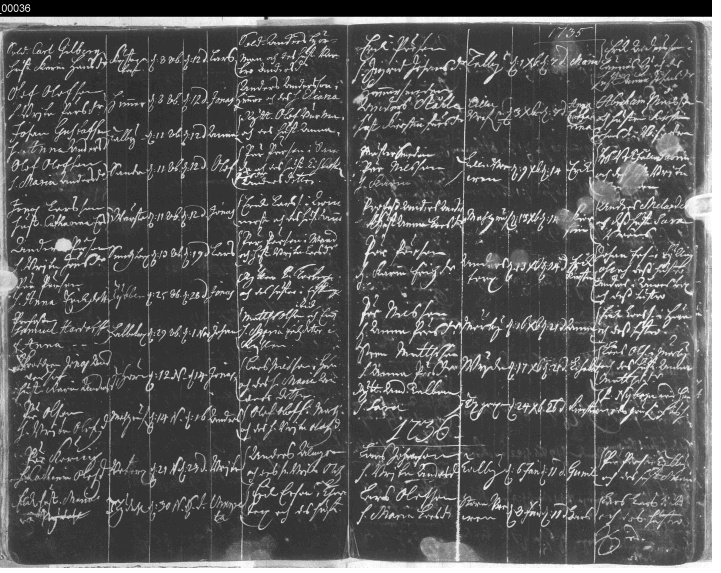
\includegraphics[scale=1.0]{resources/Edited/Orig_processed/img_S3HT-64P3-2GW.jpg}
        \caption{...}
        % \label{fig:jump_prob}
    \end{subfigure}
    \begin{subfigure}[c]{1.0\textwidth}
        \centering
        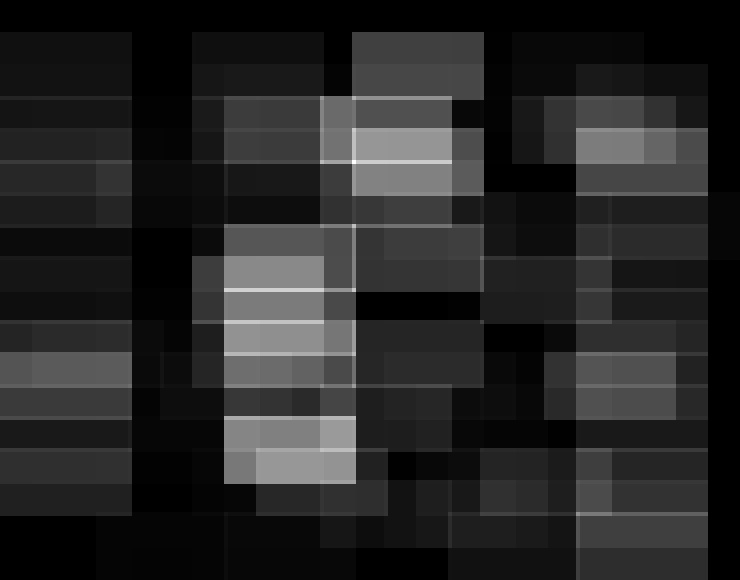
\includegraphics{resources/Edited/Orig_att/att_S3HT-64P3-2GW.jpg}
        \caption{The ...}
        % \label{fig:jump_log_counts}
    \end{subfigure}
    \caption{Caption...}
    \label{fig:my_label}
\end{figure}

We hypothesized that the network had learned other signals than the handwritten year. To test our hypothesis, we took five images from the main test set and edited them so they no longer contained any handwritten years. When running the base2 model on the five images, the predictions were exactly the same as before. The attention matrix was also almost identical with and without the handwritten year. One of these five images and the corresponding attention are visualized in figure \ref{fig:edited}.

Because the network has not seen any of these five images during training, it must have learned to recognize the handwriting of the individual scribe who wrote the book. This is likely one of the reasons why the accuracy is so much lower for our second test set, because the model has not been trained to recognize any handwriting from that dataset.

So it appears that at least for some pages, the network makes the right prediction, not because it can read the year digits, but because it recognizes the style of the handwriting. It is not what we intended the network to learn, but it nevertheless shows the potential of deep learning that the models can even learn to recognize handwriting styles.
